\documentclass[12pt]{article}
\usepackage[margin=1in]{geometry}
\usepackage{amsmath,amsthm,amssymb}
\usepackage{enumitem}
\usepackage{xspace}
\usepackage{tikz}
\usepackage{graphicx}
\graphicspath{ {./imgs/} }
\usepackage{underscore}
% \usetikzlibrary{matrix,arrows,decorations.pathmorphing,cd}
\setlist{
  listparindent=\parindent,
}
\usepackage{pgfplots}
\pgfplotsset{width=10cm,compat=1.9}
\usepackage{float}
\usepackage{polynom}
\usepackage{hyperref}
\expandafter\def\expandafter\UrlBreaks\expandafter{\UrlBreaks%  save the current one
  \do\a\do\b\do\c\do\d\do\e\do\f\do\g\do\h\do\i\do\j%
  \do\k\do\l\do\m\do\n\do\o\do\p\do\q\do\r\do\s\do\t%
  \do\u\do\v\do\w\do\x\do\y\do\z\do\A\do\B\do\C\do\D%
  \do\E\do\F\do\G\do\H\do\I\do\J\do\K\do\L\do\M\do\N%
  \do\O\do\P\do\Q\do\R\do\S\do\T\do\U\do\V\do\W\do\X%
  \do\Y\do\Z}
\newcommand{\qq}{\noindent\textbf{Q:} }
\newcommand{\N}{\mathbb{N}}
\newcommand{\Z}{\mathbb{Z}}
% various useful symbols defined here:
\newcommand{\np}{\textsc{NP}\xspace}
\newcommand{\conp}{\textsc{coNP}\xspace}
\newcommand{\p}{\textsc{P}\xspace}
\newcommand{\twosat}{\textsc{2-Sat}\xspace}
\newcommand{\threesat}{\textsc{3-Sat}\xspace}
\newcommand{\vc}{\textsc{VertexCover}\xspace}
\newcommand{\is}{\textsc{IndependentSet}\xspace}
\newcommand{\nphard}{\textsc{NP-hard}\xspace}
\newcommand{\npcomplete}{\textsc{NP-complete}\xspace}
\newsavebox{\wideeqbox}
\newenvironment{proof-idea}{\noindent{\bf Proof Idea}\hspace*{1em}}{\qed\bigskip}
\newenvironment{wideeq}
  {\begin{displaymath}\begin{lrbox}{\wideeqbox}$\displaystyle}
  {$\end{lrbox}\makebox[0pt]{\usebox{\wideeqbox}}\end{displaymath}}


\makeatletter
\renewcommand*\env@matrix[1][\arraystretch]{%
  \edef\arraystretch{#1}%
  \hskip -\arraycolsep
  \let\@ifnextchar\new@ifnextchar
  \array{*\c@MaxMatrixCols c}}
\makeatother

\newtheorem*{theorem}{Theorem}

\newtheorem*{prop}{Proposition}
\newtheorem*{conjecture}{Conjecture}

\theoremstyle{remark}
\newtheorem*{note}{Note}

\theoremstyle{remark}
\newtheorem*{remark}{Remark}

\newenvironment{must-show}{\noindent{\bf Must Show:}\hspace*{0.5em}}{\qed\bigskip}


\title{Programming Languages Theory Notes}
\author{Jae Tak Kim
}
\date{Fall 2020}

\begin{document}

\maketitle
\tableofcontents
\newpage

\section{Introduction}
\textit{Source:} Isil Dillig -- A Gentle Introduction to Program Analysis
\subsection{Overview}

\subsubsection{What is a typical static analysis question?}
Given source code of program $P$ and desired property $Q$, does $P$ exhibit $Q$ in \textit{all possible executions}?

\subsubsection{Soundness vs Completeness?}
In formal logic, an expression is sound if whenever the premise is true, the conclusion is also aways true. There's no guarantees about the conclusion if the premise is false. In the case of static analysis, the premise is that the program is unsafe and the conclusion is that our static analysis will say the program is unsafe. Thus, if the program is really unsafe, then the analysis will \textit{always} tell us that the program is unsafe. However, it's possible that the analysis will take us it's unsafe even when the program is safe.

Our analysis is complete if our program analysis always tells us the truth. Thus, completeness is a stronger condition than soundness.

\subsubsection{Describe the inherent limitations of static analysis.}
The question of trying to see if the program has a property in every single execution is undecidable. A short proof of is uses the Rice Theorem which states that all nontrivial properties are undecidable. We can even reduce this to the halting problem. 

Thus, our static analysis will be either unsound(we definitely don't want this since we don't want our analysis to say that our program is safe when it isn't), sound but incomplete($\exists$ false positives), or non-terminating(we don't want our analysis to run forever!). Clearly, the best option is the second one, so most analysis techniques will be sound but incomplete.


\subsubsection{How do you design sound static analyses?}
\begin{figure}[h]
    \centering
    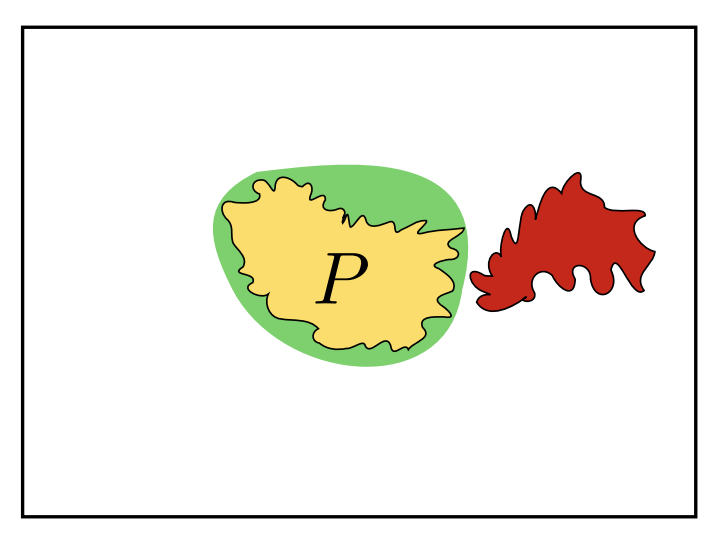
\includegraphics[scale=0.5]{overapprox}
    \caption{All possible states}
\end{figure}
We overapproximate our program behavior as little as we can. Overapproximating ensures that we never give an invalid answer. If $P$ region is the actual behavior of our program, and the green bubble is the analysis, then any states outside of the green bubble will be correctly classified. States within the green bubble but outside of the region $P$ will be false alarms (false positives). We overapproximate using abstractions so the goal of static analysis is to construct abstractions that are precise enough (few false alarms) and scale to real programs.


\subsubsection{Abstraction interpretation}
Framework for constructing sound-by-construction static analyses. Includes abstract domain, abstract function, concretization function, and abstract transformers/semantics.
\begin{figure}[h]
    \centering
    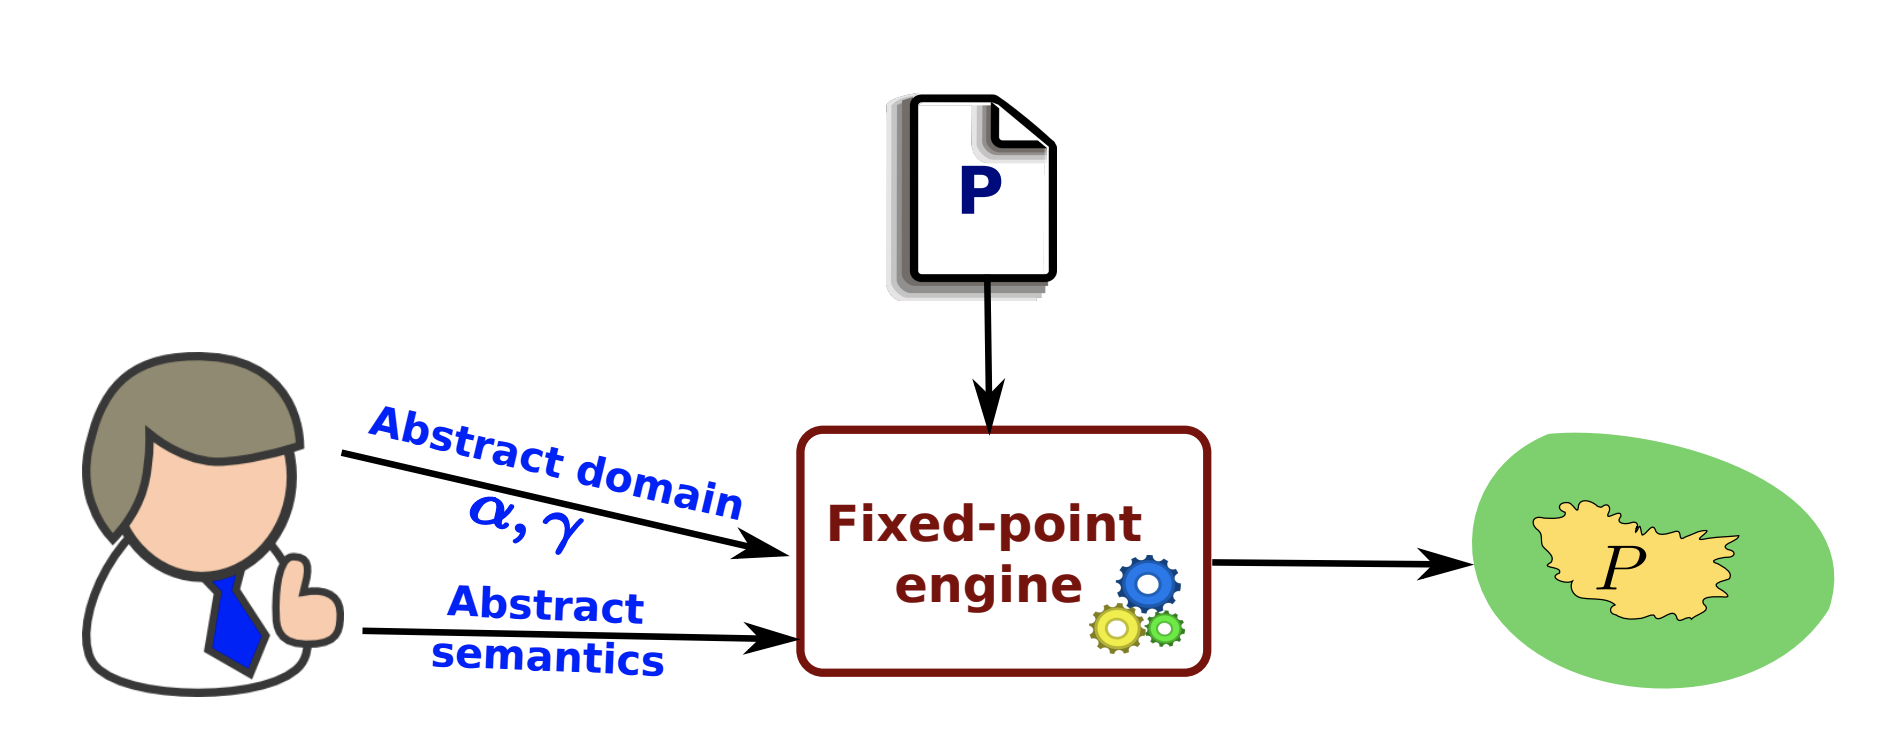
\includegraphics[scale=0.3]{analysis-process}
\end{figure}


\subsubsection{What is the idea of least-fixed point in a fixed-point computation?}
You start with an underapproximation and grow the approximation until it stops growing. This is the point where your analysis is as precise as it can be while still being sound.
\begin{figure}[h]
    \centering
    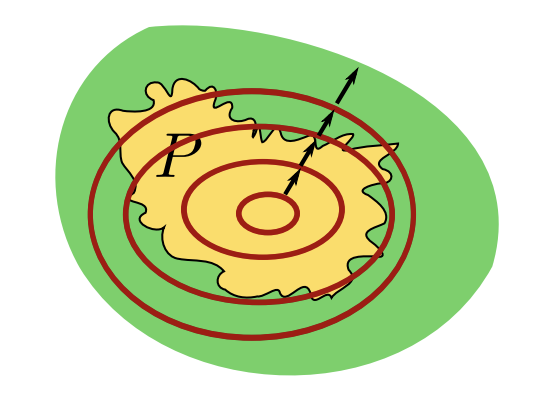
\includegraphics[scale=0.5]{least-fixed-point.png}
\end{figure}

\section{Lattice Theory}
\subsection{Equations and Fixed-Points}
\subsubsection{What is the fixed-point theorem and the general idea of the proof?}
\begin{theorem}
    In a lattice $L$ with finite height, every monotone function $f$ has a unique least fixed-point given by
    \[fix(f) = \bigsqcup_{i \geq 0} f^i (\bot)\]
\end{theorem}
\begin{proof-idea}
Because $\bot$ is the unique smallest element, we can get a chain of inclusions. Since the lattice is of finite height, it must stop somewhere, and this shows that for some $i$, $f^i(\bot) \sqsubseteq f^{i+1}(\bot)$, making this a fixed-point. We can make an argument with a least fixed-point $x$ that because $\bot \sqsubseteq x$, $f^i(\bot) \sqsubseteq x$ as well, showing that this is indeed the least fixed-point. It is unique by the fact that the partial order relation is anti-symmetric.
\end{proof-idea}

% \begin{enumerate}
%     \item What is a typical static analysis question?
%     \item Soundness vs Completeness?
%     \item Describe the inherent limitations of static analysis.
%     \item How do you design sound static analyses?
% \end{enumerate}

\end{document}